Ogni problema è stato valutato assegnando un grado di severità da 0 a 4:
\begin{itemize}
  \item 0: Non è un problema di usabilità
  \item 1: Problema accessorio
  \item 2: Problema secondario
  \item 3: Problema rilevante
  \item 4: Catastrofe di usabilità
\end{itemize}
Nel grafico seguente è riportata la distribuzione dei problemi per grado di severità:
\begin{figure}[H]
  \centering
  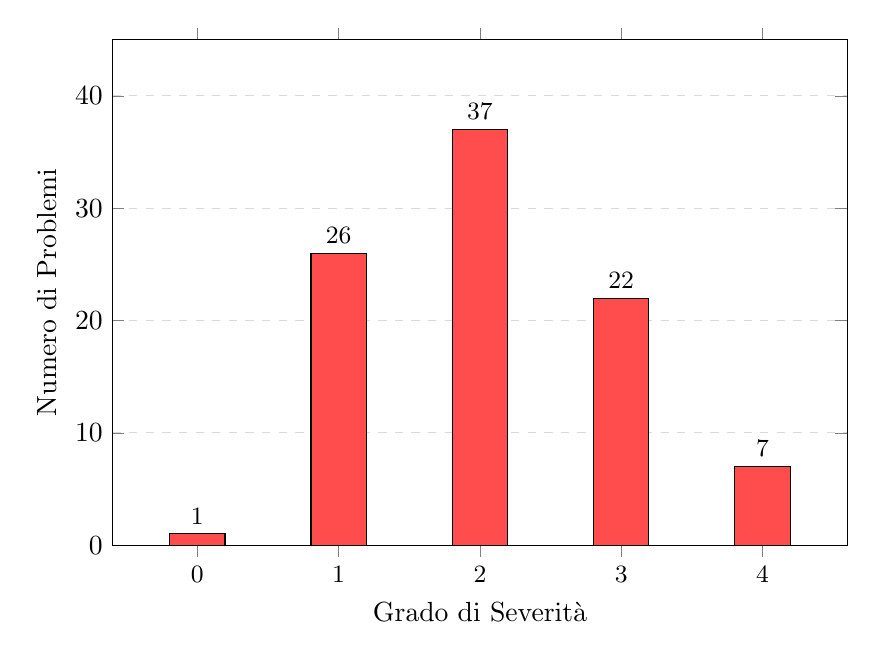
\begin{tikzpicture}
    \begin{axis}[
        ybar,
        bar width=20pt,
        width=0.9\textwidth,
        height=8cm,
        symbolic x coords={S0, S1, S2, S3, S4},
        xtick=data,
        xticklabels={0, 1, 2, 3, 4},
        x tick label style={font=\small},
        xlabel={Grado di Severità},
        ylabel={Numero di Problemi},
        ymin=0,
        ymax=45,
        ymajorgrids=true,
        grid style={dashed, gray!30},
        enlarge x limits=0.15,
        nodes near coords,
        every node near coord/.style={font=\small, color=black},
      ]
      \addplot+[ybar, fill=red!70, draw=black] coordinates {
        (S0,1)
        (S1,26)
        (S2,37)
        (S3,22)
        (S4,7)
      };
    \end{axis}
  \end{tikzpicture}
  \label{fig:severita-problemi}
  \caption{Classificazione dei problemi riscontrati rispetto al grado di severità assegnato.}
\end{figure}

La maggior parte dei problemi identificati (37 su 93, pari a circa il 40\%) rientra nella categoria di severità 2 (problemi secondari), seguita dai problemi accessori di 
severità 1 (26, pari a circa il 28\%). I problemi di severità 3 e 4, che richiedono interventi prioritari, rappresentano complessivamente circa il 31\% del totale (29 problemi). 

La distribuzione suggerisce che il sistema presenta principalmente problematiche di entità moderata, ma non mancano criticità rilevanti che dovranno essere affrontate nelle fasi successive di sviluppo.